At the end of Summer 2010, Oliver Hoidn and Perry Ellis had determined that the optimal number of OPSS-PEG-antibody (OPAb) molecules per nanosphere was approximately 2000; however, there were significant concerns as to whether the OPSS-PEG-NHS (OPN) was successfully binding to the lysines on the antibody, or whether monolayer formation was simply the result of the antibodies binding to the nanospheres via van der Waals forces. The OPN reacts with a lysine by substituting the nitrogen atom in the NHS ester for the nitrogen atom on the functional group of the lysine (and their respective attached molecules, by proxy). A diagram of this reaction is shown in \autoref{nhsreaction}.

\begin{figure}[htbp]
\centering
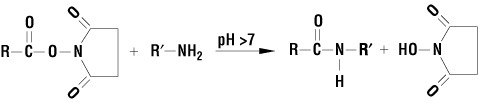
\includegraphics[keepaspectratio,width=\textwidth,height=0.75\textheight]{NHSreaction.jpg}
\caption{Schematic diagram of the OPN+antibody$\to$OPAb reaction. \textbf{R} represents the OPSS-PEG, and \textbf{R'} represents the antibody. The reaction is favored in basic conditions. From ~\citep{nhsreaction}}
\label{nhsreaction}
\end{figure}



Although the reaction requires a basic pH ($>$7) to run, basic conditions also favor a competing reaction, in which hydrolysis occurs and the NHS ester is replaced with a hydroxyl group. This renders the molecule unable to bind to antibodies, and the half-life of the hydrolysis reaction can be on the order of minutes at pH 8~\citep{nhshalflife}. Consequently, there was a concern that a large portion of the OPN used in the OPN+antibody$\to$OPAb reaction was not binding to the antibody.

Fortunately, a direct physical measurement can be used to quantify the hydrolysis of the NHS ester. The free NHS ester in solution absorbs at 260 nm much more strongly than the bound ester~\citep{Miron_Wilchek_1982}. Therefore, the Cary 5000 UV-Vis Spectrophotometer was used to monitor the absorption at 260 nm over the course of several hours. The results of this measurement are shown in \autoref{nmabsorption}.

\begin{figure}[htbp]
\centering
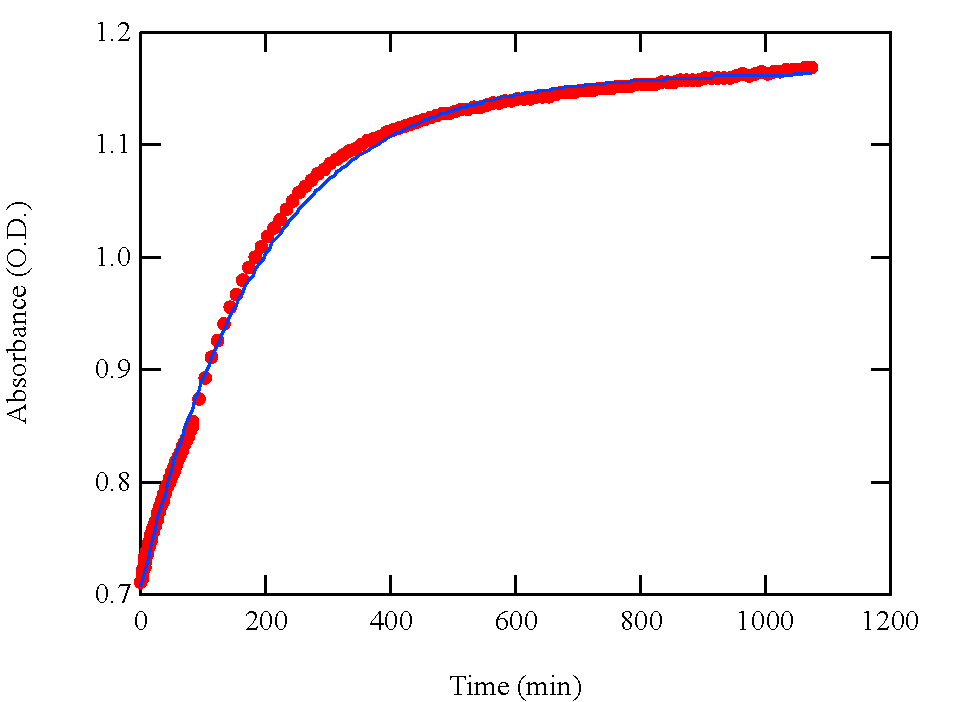
\includegraphics[keepaspectratio,width=4in,height=0.75\textheight]{NHShydro.pdf}
\caption{Plot of the absorbance of the OPN solution over time. The reaction rate seems to be proportional to concentration, giving a simple first-order rate law. The lower density of points at \ensuremath{\sim}80 minutes occurred because the spectrophotometer was set to record a spectrum every 10 minutes rather than every 1 minute. The blue line displays a fit to $A = C_1 + C_2\, e^{-C_3 t}$. The fitted values were $C_1=1.16$, $C_2=-0.458$, and $C_3=0.00523$}
\label{nmabsorption}
\end{figure}



Based on the coefficient of the exponent, $C_3=0.00523\mathrm{s^{-1}}$, we can calculate that the half-life of NHS ester hydrolysis at pH 7.5 is \[\tau_{1/2}=\frac{\ln 2}{C_3} = 133\mathrm{\,min}\]
or about two hours.

Two conclusions can be drawn from this: first, there is very little danger of having no bound NHS remaining when the protein is added, since that should occur at the most 10 minutes after the OPN solution is created (and will most likely be less than five minutes after solution creation). Second, this confirms the need to incubate the protein with the OPN overnight. Since both hydrolysis of the NHS and the reaction with the lysine work on a similar mechanism, their rates can be expected to be comparable. Thus, in order to create as much OPAb as possible, at least four hydrolysis half-lives are necessary to achieve $>90\%$ yield. However, since the hydrolysis is nontrivial on that time scale, we will use OPN should be used in a factor of 2 excess in order to facilitate maximal protein binding. Therefore, in the PEGylation procedure, we will use 2,000 antibodies per Au nanosphere and 4,000 OPN molecules per nanosphere (see \autoref{app:pegylation}).
